\documentclass{article}
\usepackage{graphicx}
\usepackage[fleqn]{amsmath}
\usepackage{pdfpages}
\usepackage[a4paper, margin=2cm]{geometry}
\newcommand{\comment}[1]{}
\begin{document}
\title{Practical 2}
\author{Janco Spies, u21434159}
\maketitle
\section*{Task 1}
\begin{itemize}
    \item[1.3] The Template Method pattern has been implemented.
\end{itemize}

\section*{Task 2}
\begin{itemize}
    \item[2.4] 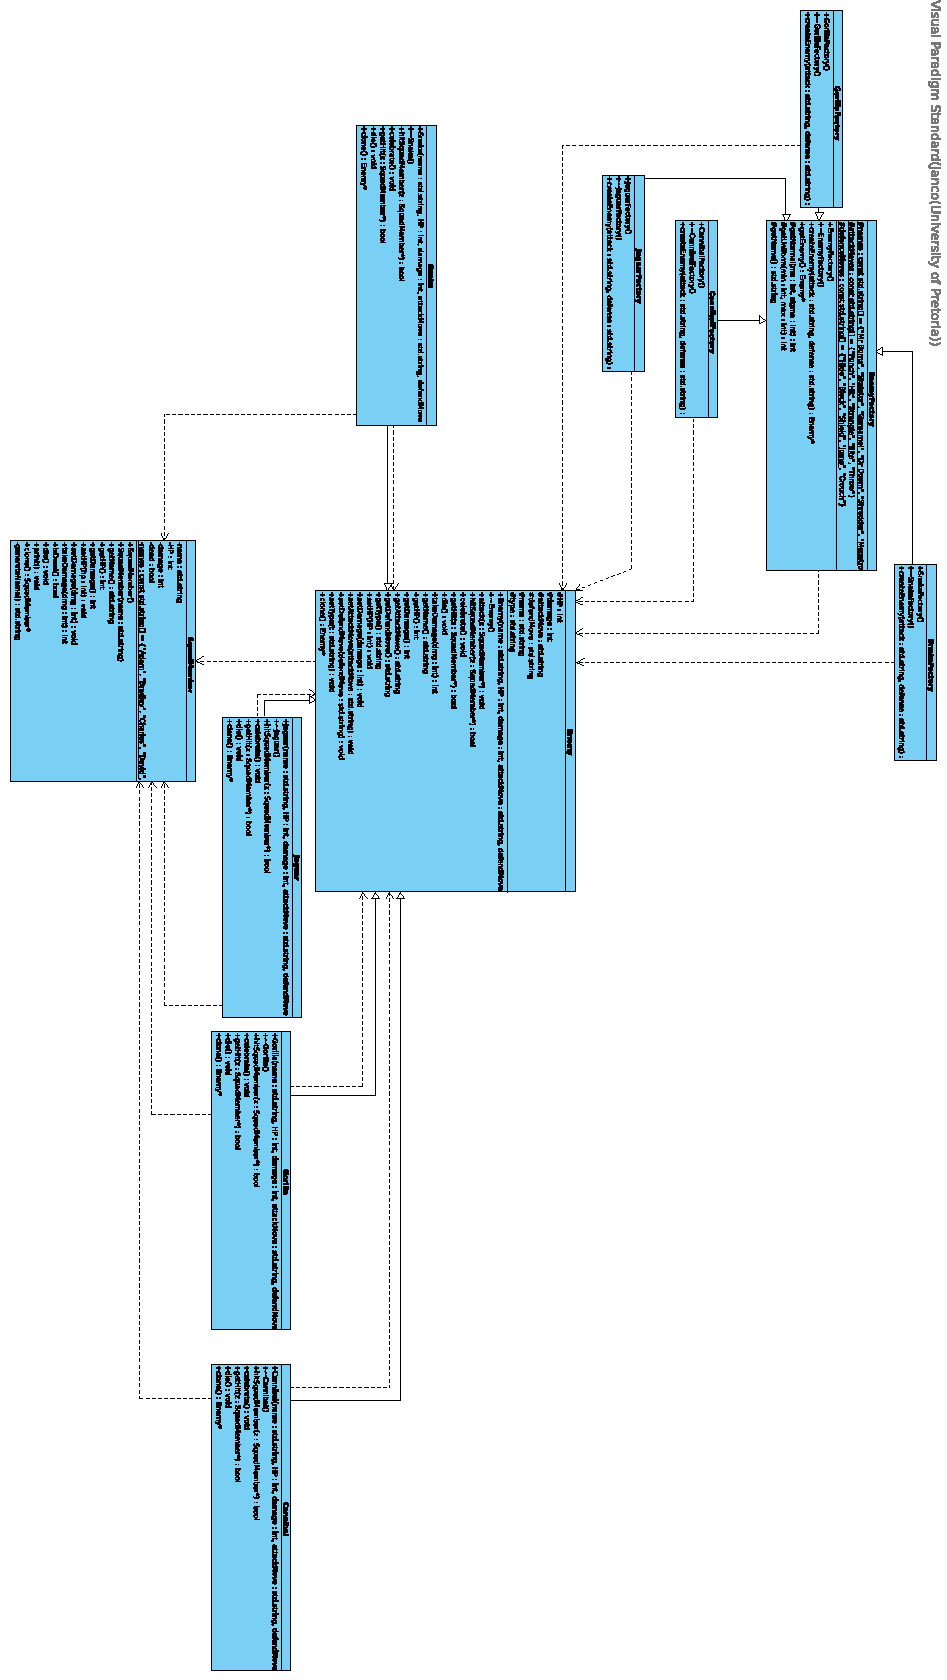
\includepdf[pages=-]{Task2_4.pdf}
    \item[2.5] 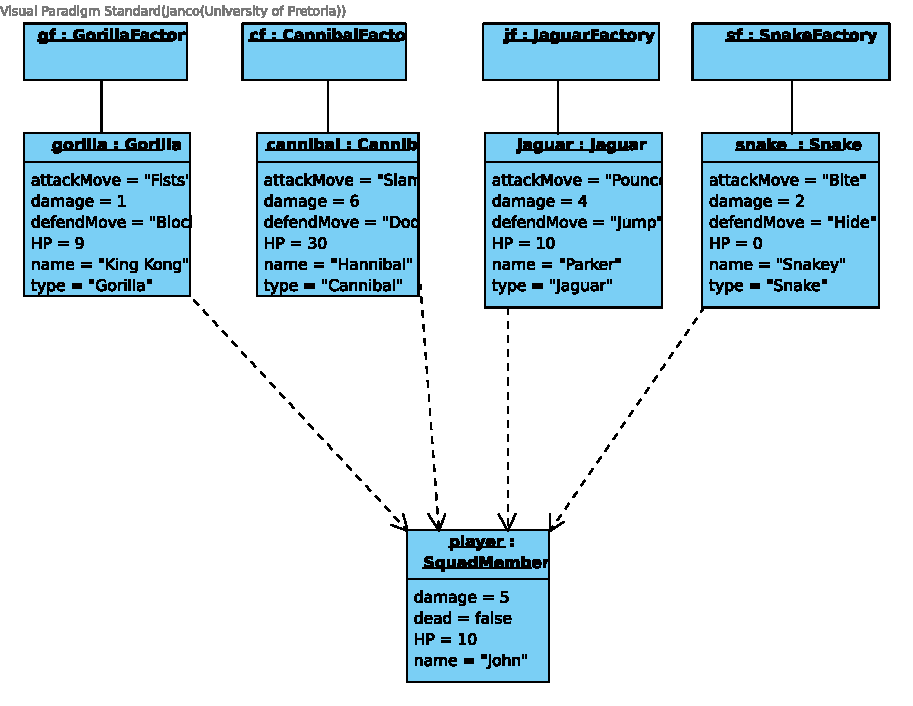
\includepdf[pages=-, scale=0.45]{Task2_5.pdf}
    \item[2.6] The Gang of Four Factory Method pattern is realized in my implementation with the following participants:\\
        \textbf{Creator}: EnemyFactory\\
        \textbf{ConcreteCreator}: CannibalFactory, JaguarFactory, SnakeFactory and GorillaFactory\\
        \textbf{Product}: Enemy\\
        \textbf{ConcreteProduct}: Cannibal, Jaguar, Snake and Gorilla\\~\\
        The Gang of Four Factory Method pattern is realized in my implementation with the following methods:\\
        \textbf{anOperation()}: getEnemy()\\
        \textbf{factoryMethod()}: createEnemy()\\
    \item[2.7] The Factory Method design pattern together with the Template Method design pattern has been implemented.  
\end{itemize}

\section*{Task 4}
\begin{itemize}
    \item[4.2] a) The fist way I expanded my game was by adding a checkpoint save system 
                    which allows the player to save the game at any time and then restore
                    the most recently saved checkpoint. The functions of the Memento pattern 
                    are :\\
                  \textbf{getState()}: State is set in the CheckPoint() parameterized constructor.\\
                  \textbf{setState()}: State is restored using  getter methods in the CheckPoint class.\\
                  The Game class acts as the Originator, the CheckPoint class acts as the Memento 
                  and the Backup class acts as the Caretaker. Sate is defined as the SquadMember* array
                  storing the names, HP and damage of each squad member as well as the current score.\\
                    
                b) The second way I expanded my game was by adding an undo move system 
                which allows the player to undo the last move. The functions of the Memento pattern
                are :\\
                \textbf{getState()}: State is set in the Move() parameterized constructor.\\
                \textbf{setState()}: State is restored using getter methods in the Move class.\\
                The Game class acts as the Originator, with the Move class acting as the 
                Memento and the MoveHistory class acting as the caretaker. State is defined as the 
                SquadMember* array storing the names, HP and damage of each squad member as well as the 
                current score and current enemy being faced in the encounter.\\

\end{itemize}
\end{document}